\section{扩展生成器能力}

第~\ref{sec:judge} 节把裁判可靠度视为绑定约束。现在提出其对偶的问题：一旦可靠的裁判已经可用，是什么限制了生成器\emph{使用}它的能力？首先给出一个四层约束框架（\S\ref{sec:fourlayer}），随后在真实 API 调用上验证它（\S\ref{sec:api}），最后报告能够把真实的生成器改进与裁判侧假象区分开的统计检验（\S\ref{sec:stat}）。

\subsection{四层约束框架}
\label{sec:fourlayer}

第~4.3 节表明，自由形式的代码生成是生成器侧的绑定约束。因此
将其替换为一条四层流水线：

\begin{enumerate}
  \item \textbf{JSON 骨架生成。} 教师提示词要求输出 JSON 对象而非
        Python 代码，从而消除括号匹配与变量声明这两类失败。
  \item \textbf{确定性渲染。} 由模板化渲染器把骨架转换为 Z3 Python
        代码，因此输出在构造上即语法合法。
  \item \textbf{符号反馈。} Z3 错误码被映射为命名补救措施。该映射已实现并有单元测试，
        但实验框架对每个任务只构造一次教师提示词，且传入的是
        \texttt{extra\_constraints=None}，因此提示在下文运行中并未到达模型；
        那些运行真正起作用的是重试预算。
  \item \textbf{课程控制器。} 子档位控制器（连续五轮有效任务率 $> 0.80$ 时提升、
        连续三轮低于 $0.50$ 时降低）已实现并有单元测试
        （\texttt{scripts/difficulty\_controller.py}），但未接入任何一个轮次循环：
        下文的验证把每个等级当作固定因子显式请求。
\end{enumerate}

四层之中，承担下文实测增益的是前两层；后两层已实现并有测试，但并未被这些运行所执行。

\subsection{真实 API 验证}
\label{sec:api}

使用真实的 DeepSeek V4 Flash API，在 240 轮（4 个条件 $\times$ 3 个层级 $\times$ 20 轮）
上验证该约束框架。各条件之间的改进情况见
图~\ref{fig:improvement_comparison}。

在该框架就位后，真实 API 下的有效任务率为 L1 = 100.0\%（80/80）、L2 = 73.8\%
（59/80）、L3 = 83.8\%（67/80）。

在 34 个无效轮次中，33 个是
\texttt{error\_code=1: LLM did not return valid JSON}——模型产出的输出完全无法解析——
另有 1 个是模式违规（不支持的变量类型）。因此，每一个无效轮次都可归因于模型，
而非框架。这是该方法诚实的下限：框架保证良构骨架会变成良构约束集，却无法保证
模型一定产出良构骨架。这也正是为什么上述比率衡量的是生成器能力，
而不是工具链本身的可靠性。

\begin{figure*}[t]
  \centering
  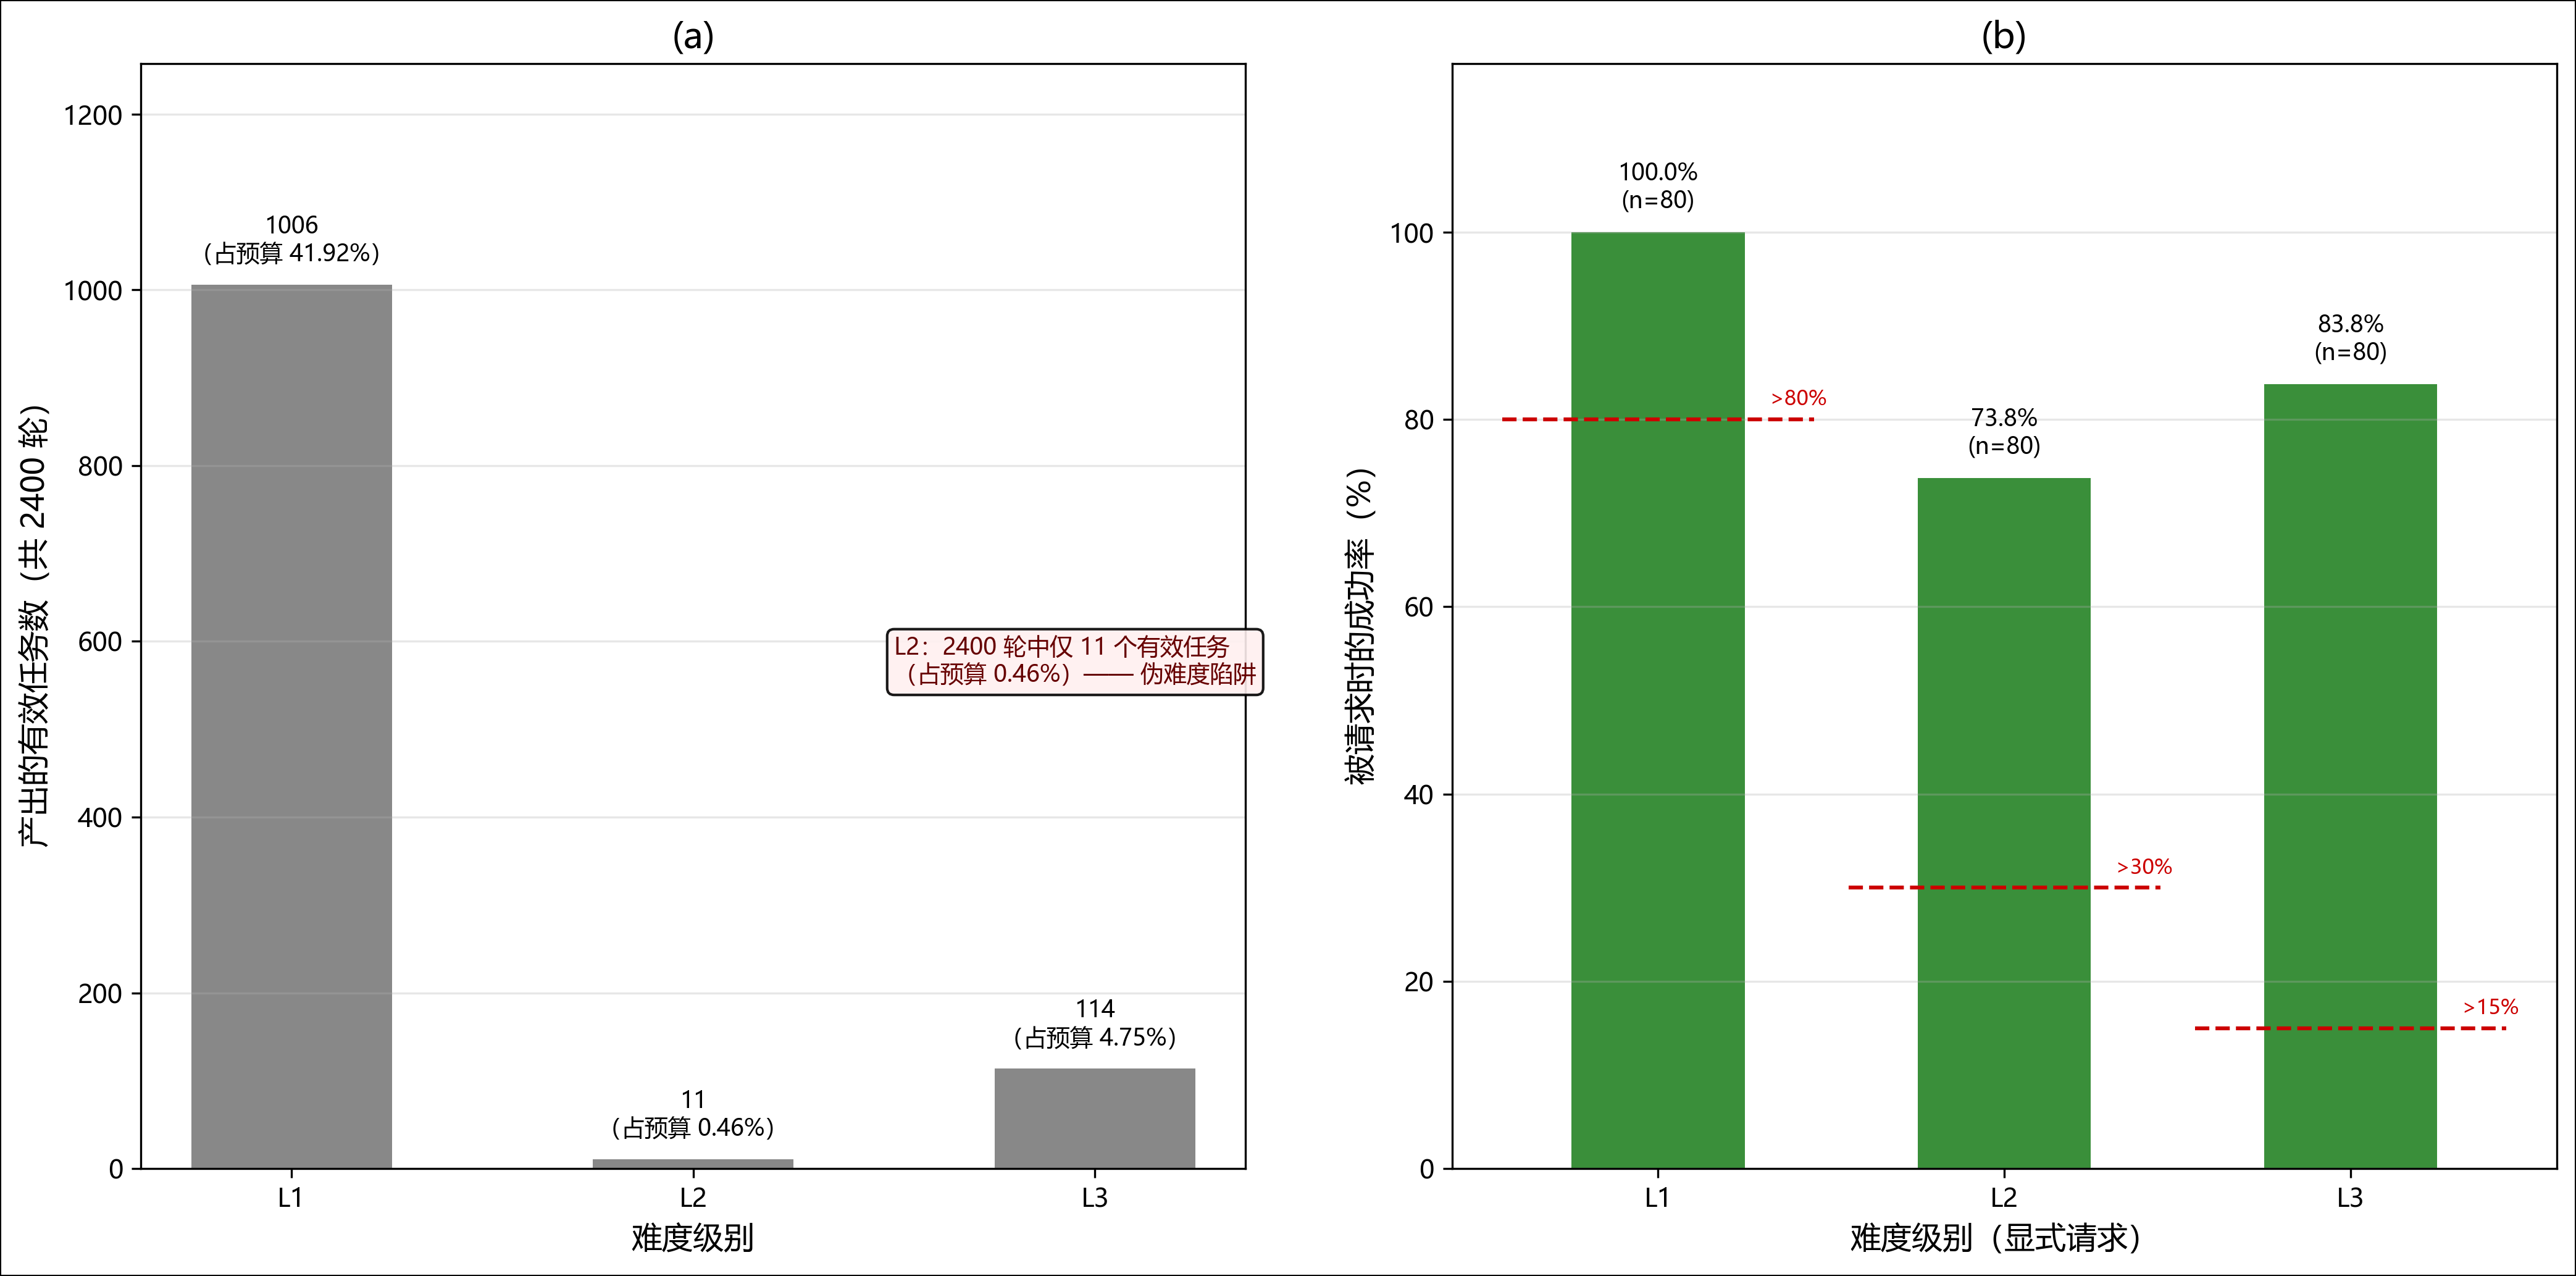
\includegraphics[width=0.7\textwidth]{figures_zh/fig6_improvement_comparison_real.png}
  \caption{在四层约束生成框架启用前/后，真实 API 上的 240 轮
  （4 个条件 $\times$ 3 个层级 $\times$ 20 轮）。采用该框架时的有效任务率为 L1 =
  100.0\%（80/80）、L2 = 73.8\%（59/80）、L3 = 83.8\%（67/80）；而旧版教师
  在 2,400 轮中仅产出 11 个有效 L2 任务与 114 个有效 L3 任务。由于两次运行的预算与
  分母不同，此处比较的是能力，而非比率。}
  \label{fig:improvement_comparison}
\end{figure*}

\subsection{统计验证}
\label{sec:stat}

\S\ref{sec:api} 中的 API 结果显示该框架提升了有效任务率，但这些结果
并未排除一种裁判侧假象：一个更干净的裁判可以提高测量到的有效性，
而生成器质量并无任何真实增益。因此，对已发布的真实 API 日志
施加 Welch 的 $t$ 检验，且不采用任何重采样流程。

\paragraph{逐条件检验。} 60 个框架轮次对 600 个旧版轮次给出：A 为
$t = 4.26$（$p = 2\times10^{-5}$，$d = 0.60$），B 为 $t = 0.82$（$p = 0.41$，$d = 0.11$）。
A 有可测量的改进，而 B 仍为零结果，这与"该框架绑定的是生成器而非裁判"相一致。
而在生成器瓶颈确实绑定的
地方，位移是决定性的：C 从 $\Delta_t = 0.8767$ 变为 $0.1500$（$t = 15.12$，$d = 2.38$），D 从 $0.9050$
变为 $0.1333$（$t = 16.83$，$d = 2.59$）。

\paragraph{口径一致的 L1 检验。} 旧版分母排除了失败轮次，因此只有 L1
可比。在该层级上，改进后的教师显示出更低的 $\Delta_t$（$0.000$ 对 $0.082$；Welch
$t = 34.61$，$p < 10^{-15}$，Cohen's $d = 1.13$，大效应量）。

\paragraph{口径注意事项。} \S\ref{sec:calibers} 的两种口径仅在对无效轮次的处理上
不同：global 口径对每个无效轮次计入 $\Delta_t = 1.0$，valid-only 口径则将其
排除。逐条件检验采用 global 口径——这是保守的选择，因为减少
无效轮次正是该框架所主张的效果。

% ===========================================================================
% 7-8
% ===========================================================================
\section{讨论}

该公式意味着，“足够可靠”并非一种绝对属性。对于一个 $\Delta_t^{\max} = 0.35$ 的
系统，可靠度为 55\% 的裁判即已够用。这重新框定了裁判稀缺问题：实际的
问题不是“能否找到一个完美的裁判？”，而是“在给定生成器
$\Delta_t^{\mathrm{gen}}$ 的前提下，系统能承受多大的容差 $\Delta_t^{\max}$？”

由此导出三项具体的部署前检查（pre-deployment check）。(1) 在控制器被允许
请求的最高难度上测量生成器的误差 $\Delta_t^{\mathrm{gen}}$。若
$\Delta_t^{\mathrm{gen}} \ge \Delta_t^{\max}$，则生成器就是瓶颈；此时改进裁判只是
白费力气。(2) 在一组留出的有效任务上测量裁判的误差；这直接给出 $\tau$。
(3) 将二者代入 $\tau_c = \sqrt{1 - 2\Delta_t^{\max}}$ 并与实测的
$\tau$ 比较。若 $\tau < \tau_c$，预期出现单调漂移；若 $\tau \ge \tau_c$，预期行为
稳定或持续改善。在的情形中，L1 扫描给出 $\tau = \tau_c = 0.55$，而完整的 2,400 轮运行
给出 $\Delta_t^{\mathrm{gen}} = 0.855$（C）与 $0.905$（D），二者均超过 $\Delta_t^{\max} = 0.6$
——这正是伪难度陷阱。

合成律还提示了一个架构方向：自进化系统应把 $\Delta_t^{\mathrm{gen}}$ 与 $\tau$ 作为
一等遥测（telemetry）暴露出来，并以 $\Delta_t^{\mathrm{gen}} < \Delta_t^{\max}$ 作为
难度升级的门控条件。四层约束框架正是其中一种实例
——它降低 $\Delta_t^{\mathrm{gen}}$，直到生成器不再耗尽整份预算，此时
$\tau_c$ 才成为一个有意义的运行阈值。

\section{结论}

着手测量的是：自进化智能体若要改进，裁判必须有多可靠。答案并非
一个固定数值，而是生成器已经花掉多少误差预算的函数：合成律
$1 - \Delta_t^{\mathrm{global}} = (1 - \Delta_t^{\mathrm{gen}})(1 - \Delta_t^{\mathrm{valid}})$
在 2{,}400 个真实 API 轮次上成立至机器精度，并给出一个不含拟合参数的
闭式解 $\tau_c = \sqrt{1 - 2\Delta_t^{\max}}$。由此可得两个结果。第一，伪难度陷阱：
一旦生成器瓶颈超出容差，任何裁判可靠度都无法挽救该循环。第二，
$\tau_c$ 并非系统的常数——一个同时具备种群博弈、蒸馏与圆桌共识的系统，
与一个最小的 Z3 锚定循环返回相同的 $\tau_c$，因为该公式只关心
生成器留下了多少预算。这把自进化问题从“增加更多机制”
重新框定为“先测量预算的分配”。

% ===========================================================================
% REFERENCES
% ===========================================================================
% 用 unsrtnat（而不是 plainnat），使文献编号按首次引用顺序排列：
% 正文中第一次 \cite 会成为 [1]。plainnat 按作者字母序编号，
% 这会让引言开篇处出现 [3]。
\bibliographystyle{unsrtnat}
\bibliography{refs}

% ===========================================================================
% APPENDICES
% ===========================================================================
\appendix

\section{完整图集}

本附录汇集完整图集以供参考。图~\ref{fig:delta_t_global}、\ref{fig:delta_t_L1_phase}、\ref{fig:difficulty_trajectory} 与 \ref{fig:tau_c_gap} 分别展示全局 $\Delta_t$ 轨迹、L1 阶段分解、难度轨迹，以及经验--解析 $\tau_c$ 差距。图~\ref{fig:analytical_fit_appendix}、\ref{fig:validity_by_level_appendix}、\ref{fig:tau_c_curve_appendix} 与 \ref{fig:delta_t_per_round_appendix} 依次补充解析拟合、分级有效任务率、$\tau$ 扫描与逐轮 $\Delta_t$ 分解。

\begin{figure*}[t]
  \centering
  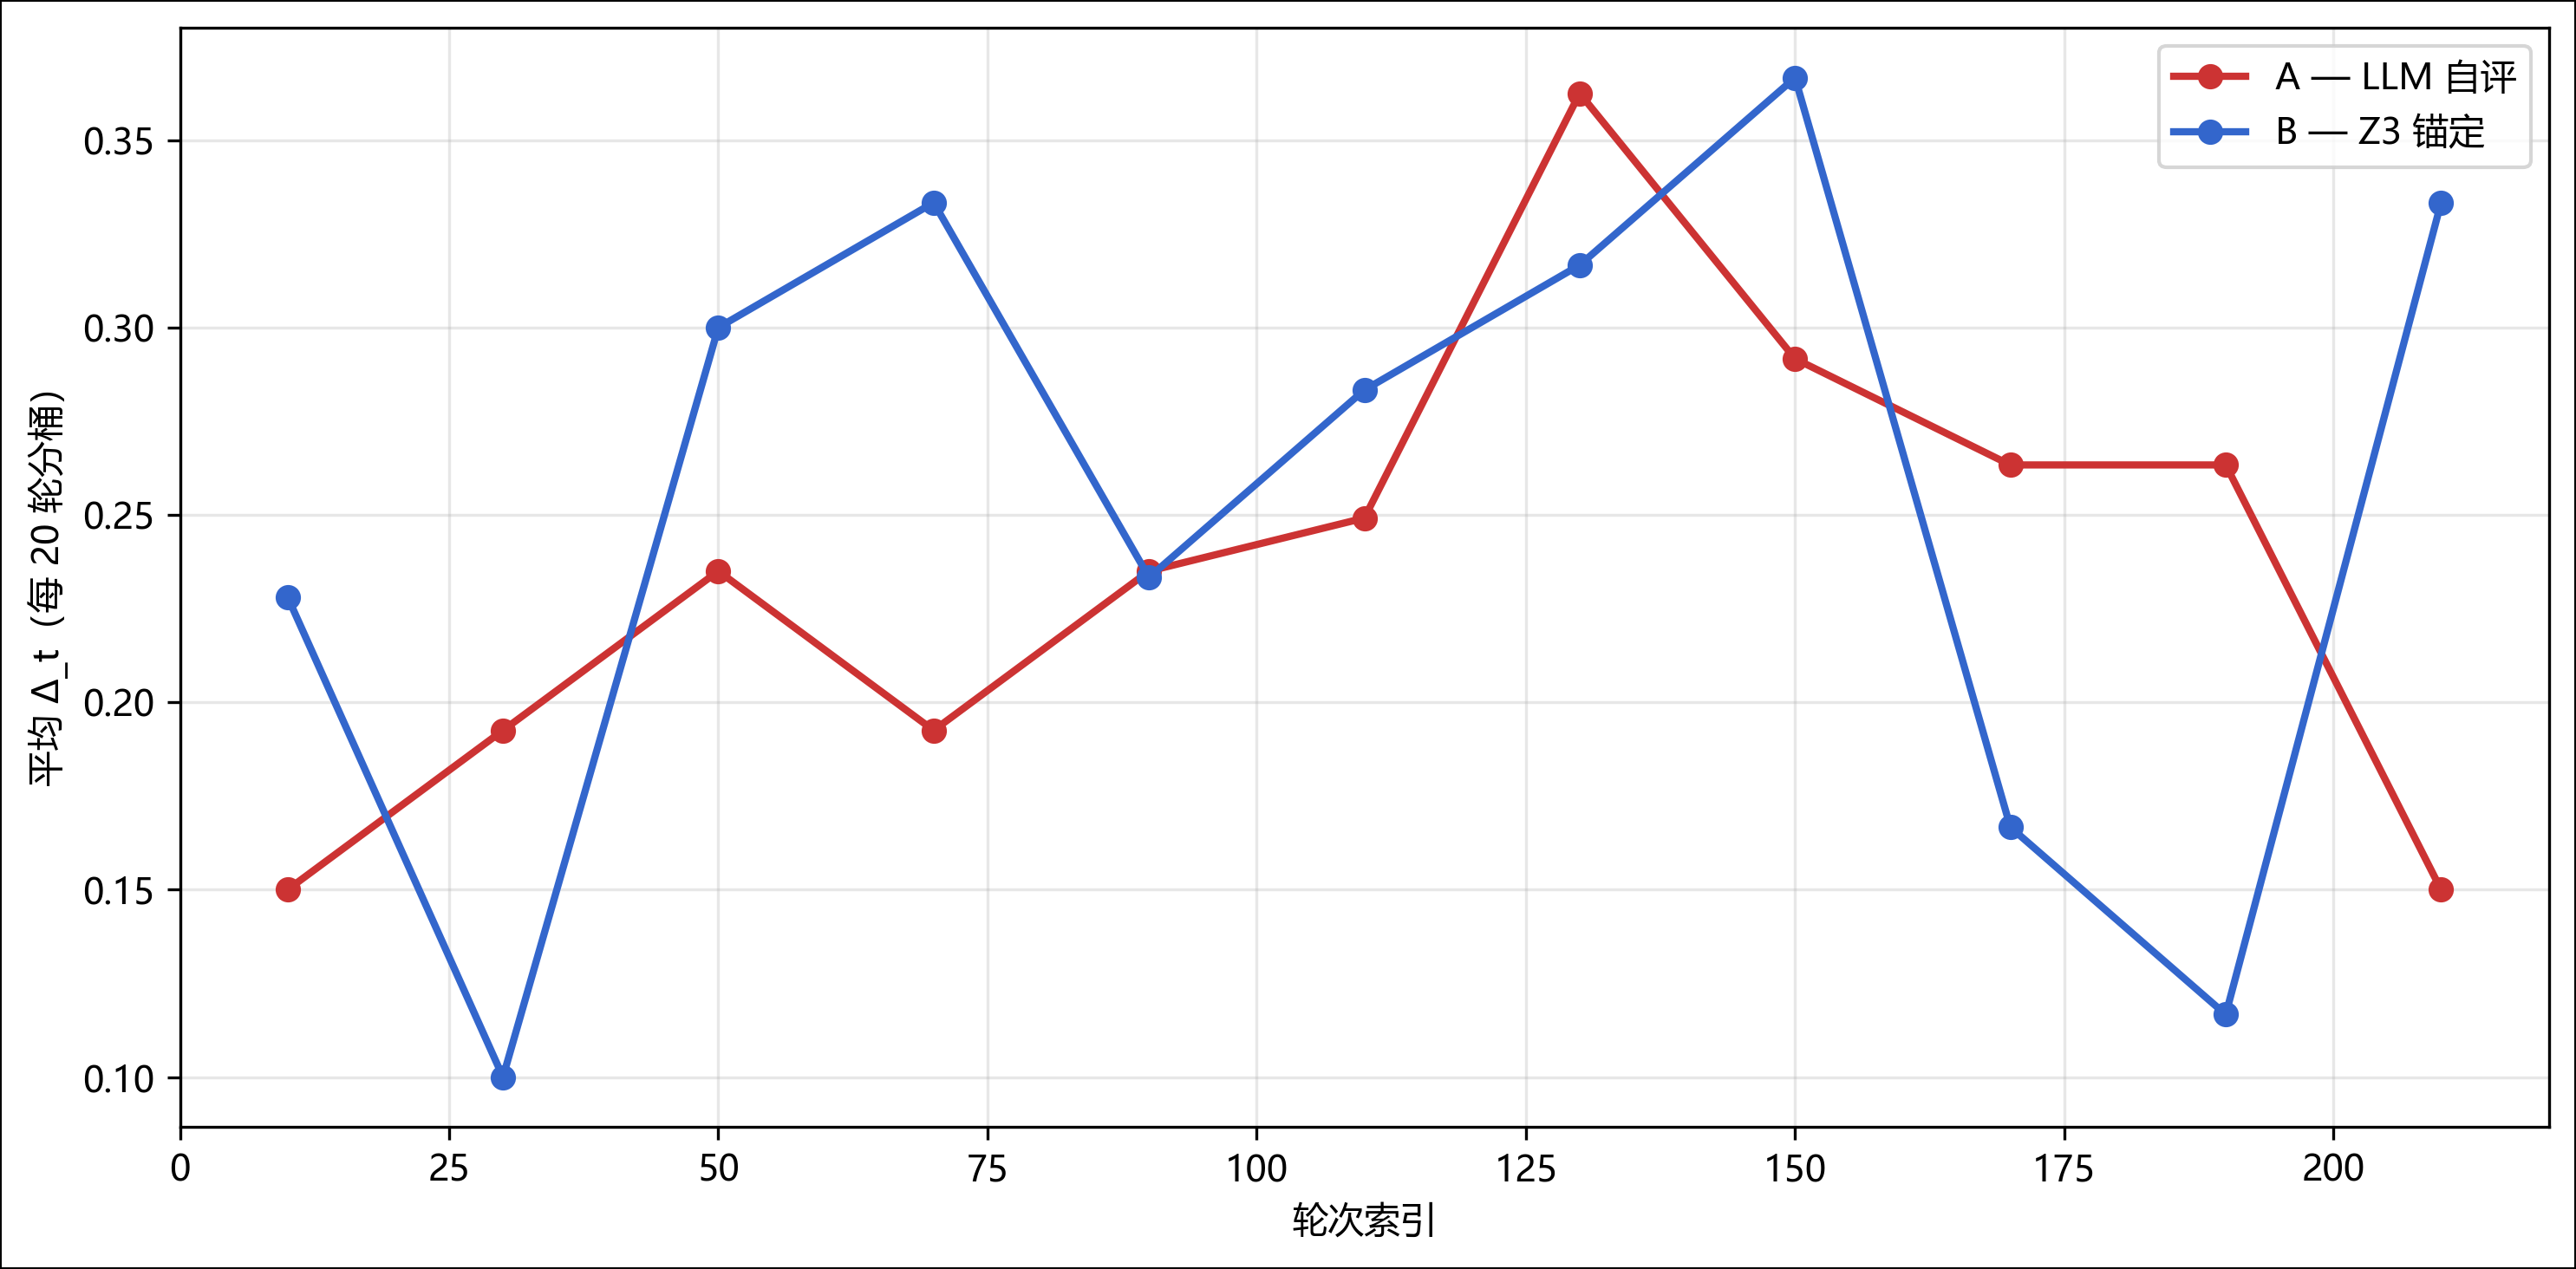
\includegraphics[width=\textwidth]{figures_zh/fig2_delta_t_AB.png}
  \caption{Global 口径的 $\Delta_t$（无效轮次编码为 $\Delta_t=1.0$）。
  条件 A 的平均值为 0.2435，条件 B 的平均值为 0.2450——二者看似
  相近，是因为 B 更高的无效率抵消了其在有效轮次上的零偏差。
  valid-only 口径（图~\ref{fig:delta_t_per_round_appendix}）隔离了裁判
  行为，是比较裁判可靠度时应采用的正确视角。}
  \label{fig:delta_t_global}
\end{figure*}

\begin{figure*}[t]
  \centering
  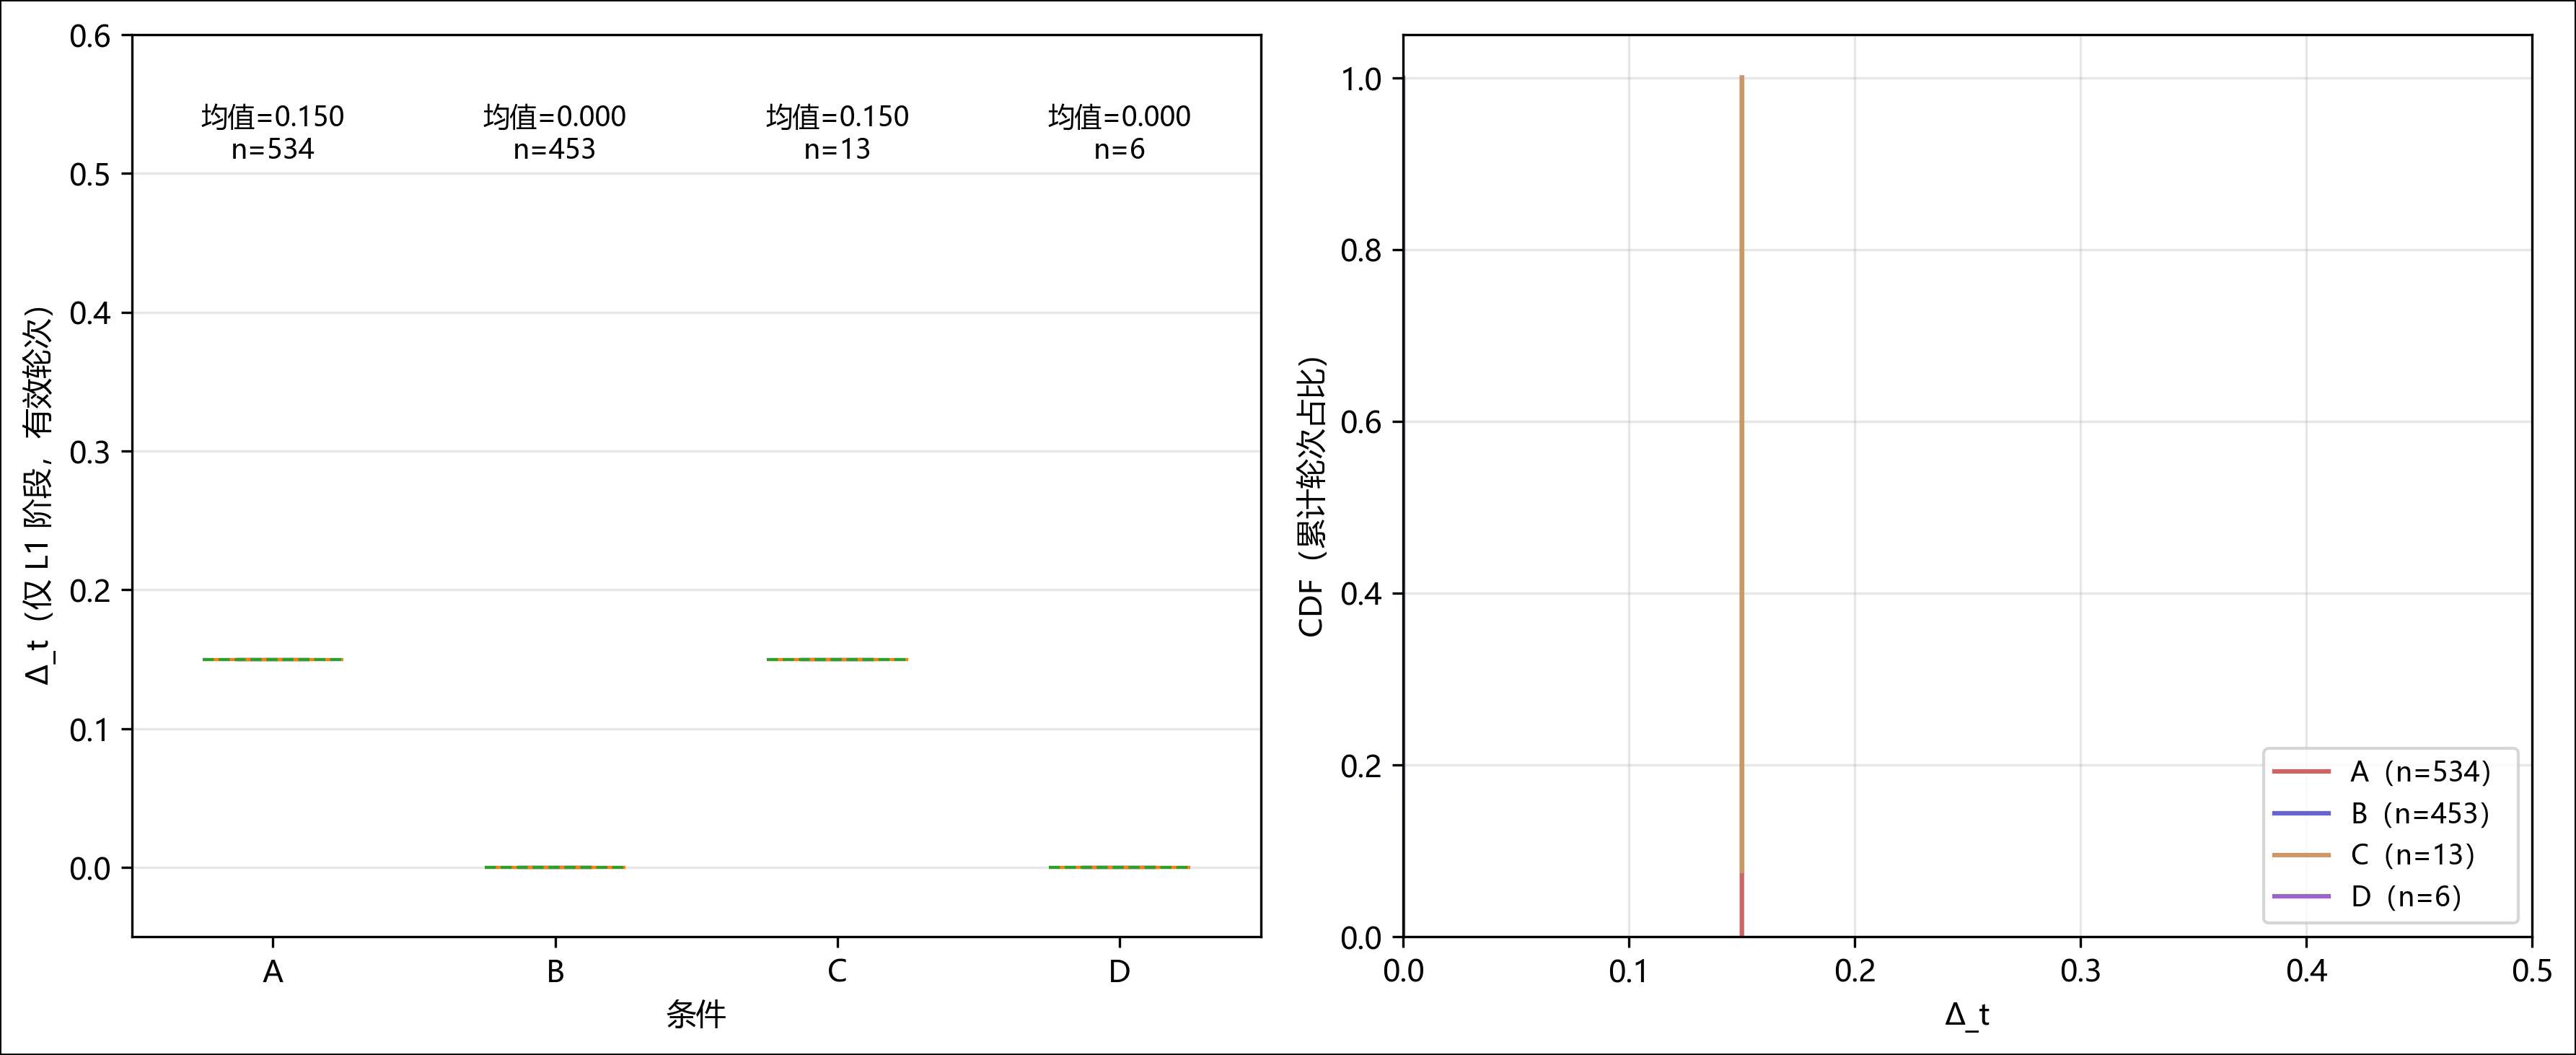
\includegraphics[width=\textwidth]{figures_zh/fig2c_delta_t_L1_only.png}
  \caption{仅限 C/D 被提升到 L2 之前的那些轮次。C/D 在 L1 阶段的 $\Delta_t$
  并\textit{不}比 A/B 更差，因此种群博弈本身并不损害性能——C/D
  后来的退化源自难度升级，而非机制中的缺陷。注意：
  C/D 的 L1 阶段样本量（$n = 13$，$n = 6$）偏小，因为难度控制器
  升级过快。“种群在 L1 上无害”这一断言只是方向性的；更大样本的
  确证留待未来工作。}
  \label{fig:delta_t_L1_phase}
\end{figure*}

\begin{figure*}[t]
  \centering
  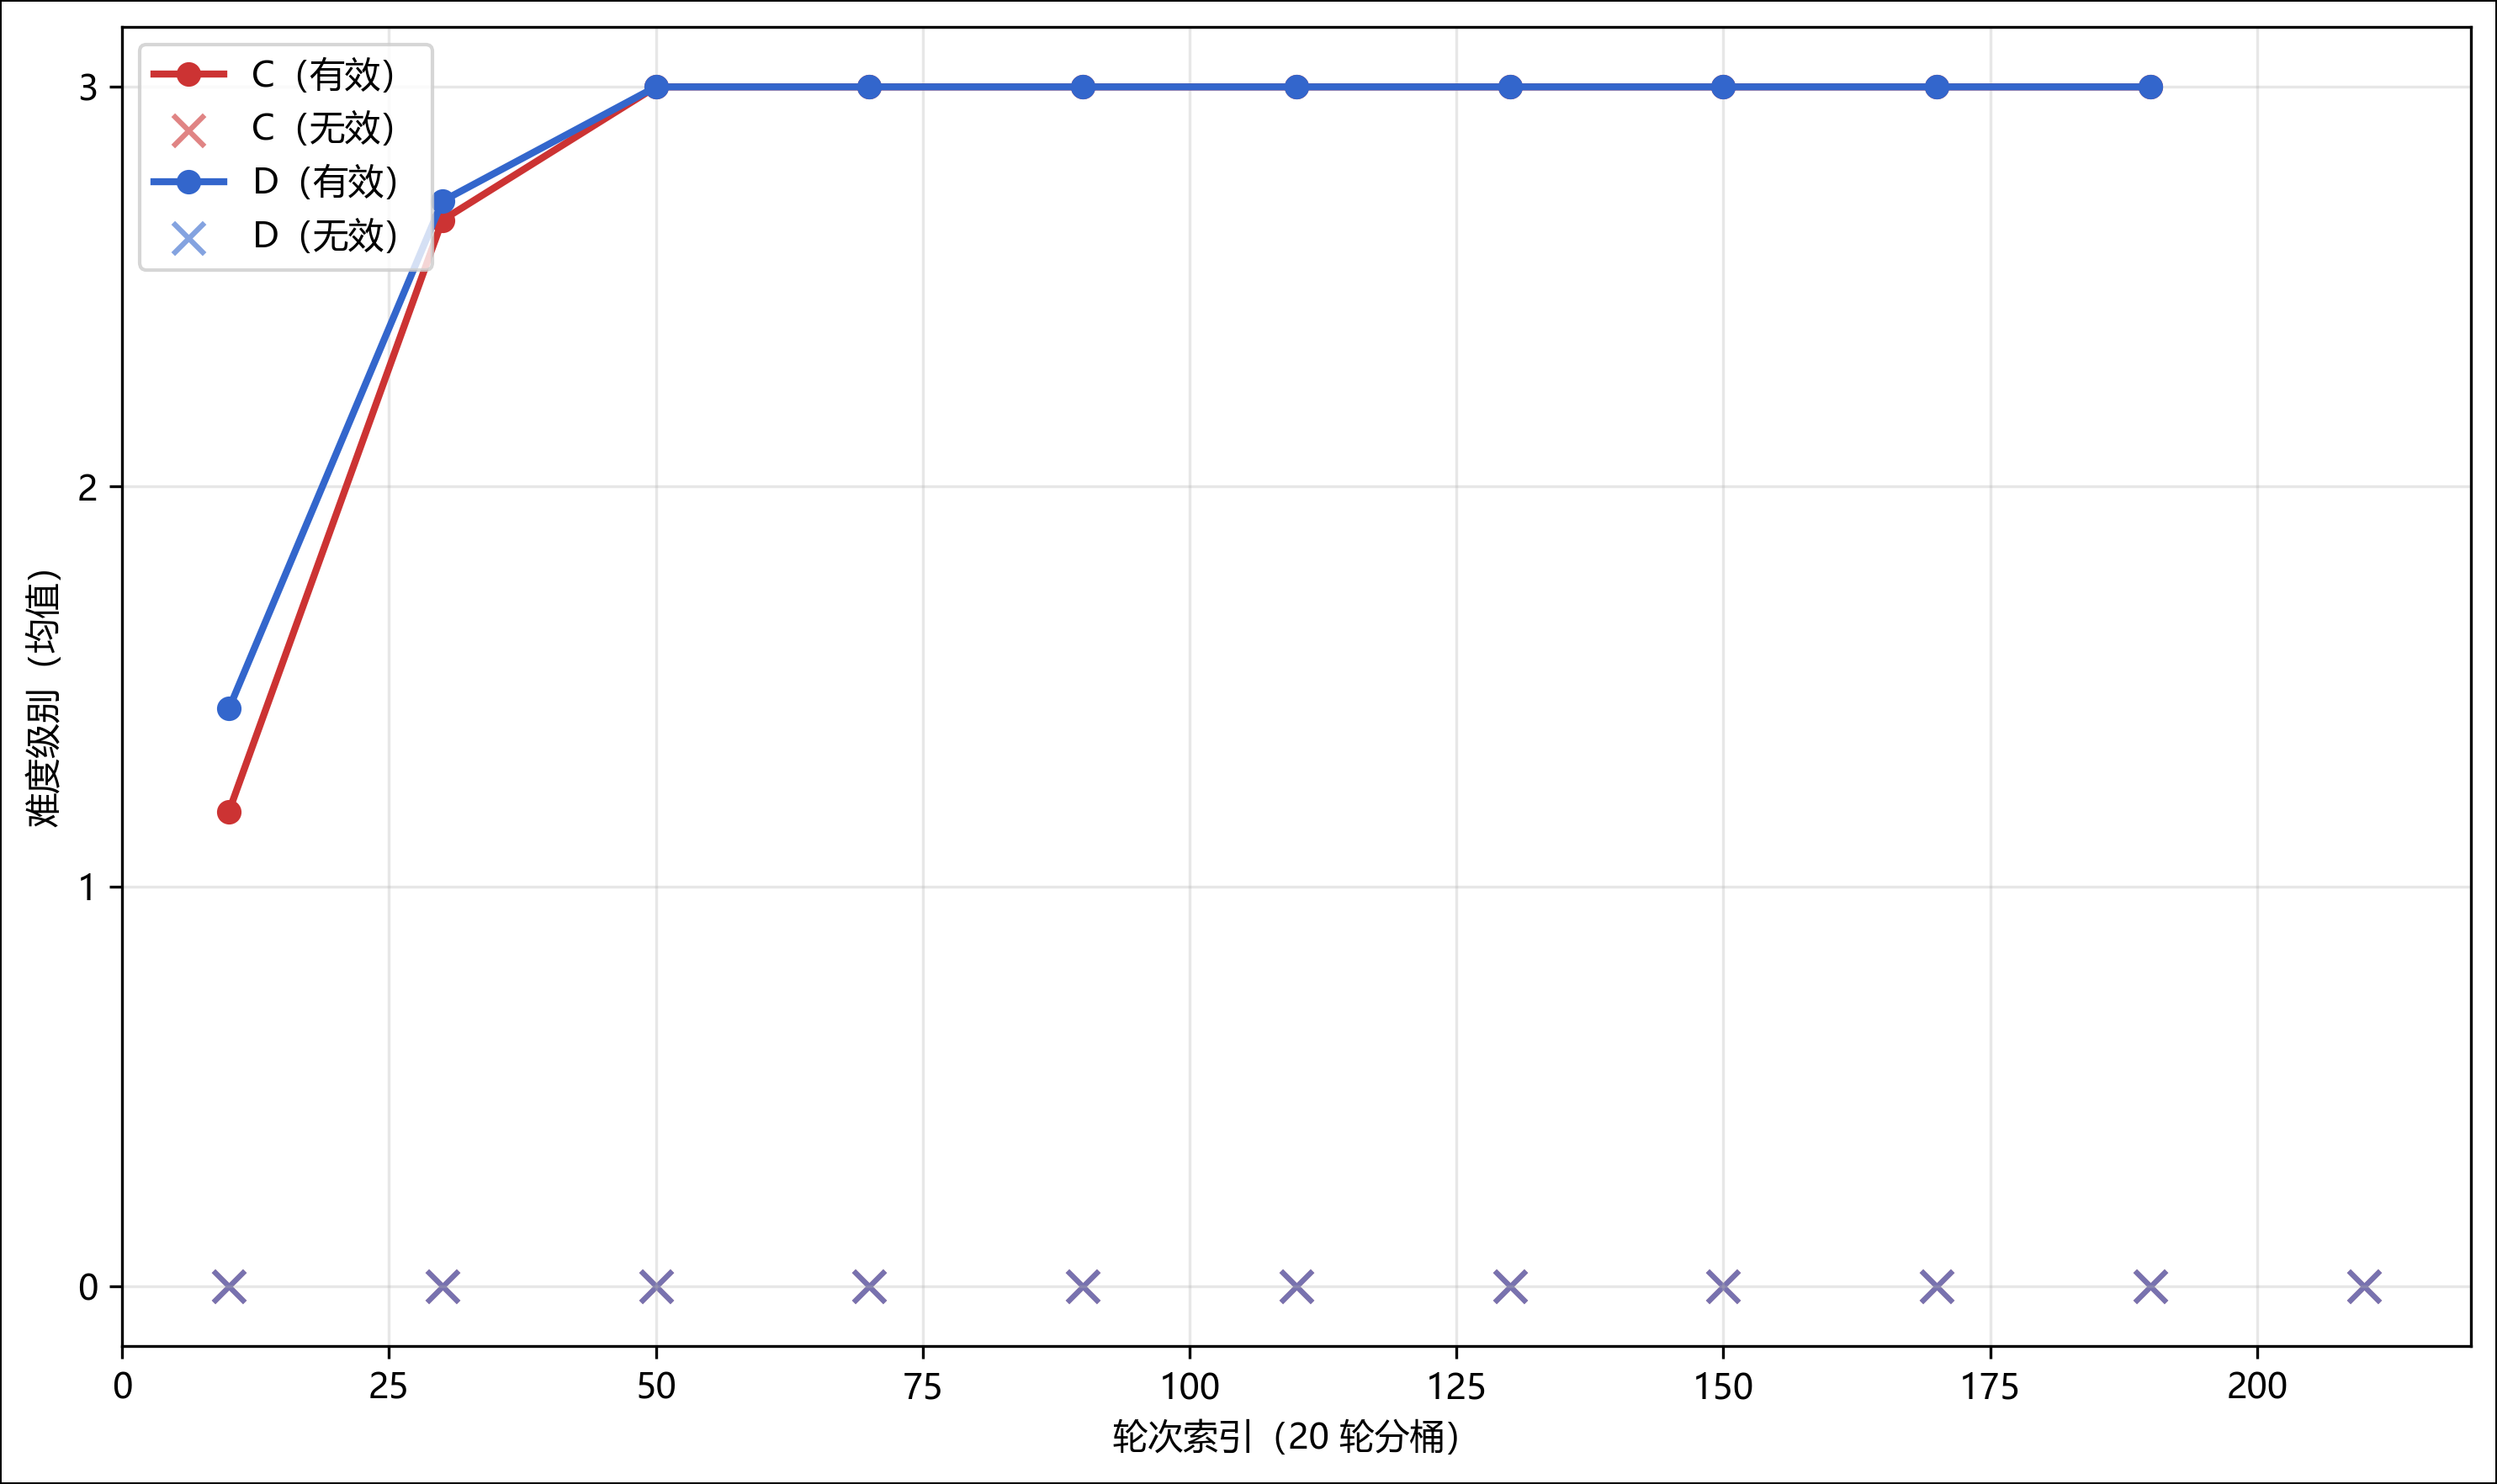
\includegraphics[width=\textwidth]{figures_zh/fig4_difficulty_trajectory.png}
  \caption{条件 C 与 D 的难度轨迹。失败在难度上\textit{并非}均匀
  分布——它们聚集在升级发生的那一刻。一旦层级被提升，
  教师持续失败，而控制器却把层级维持在高位，于是系统自以为
  在解决更难的问题，实际却把预算花在不可用的任务提案上。}
  \label{fig:difficulty_trajectory}
\end{figure*}

\begin{figure*}[t]
  \centering
  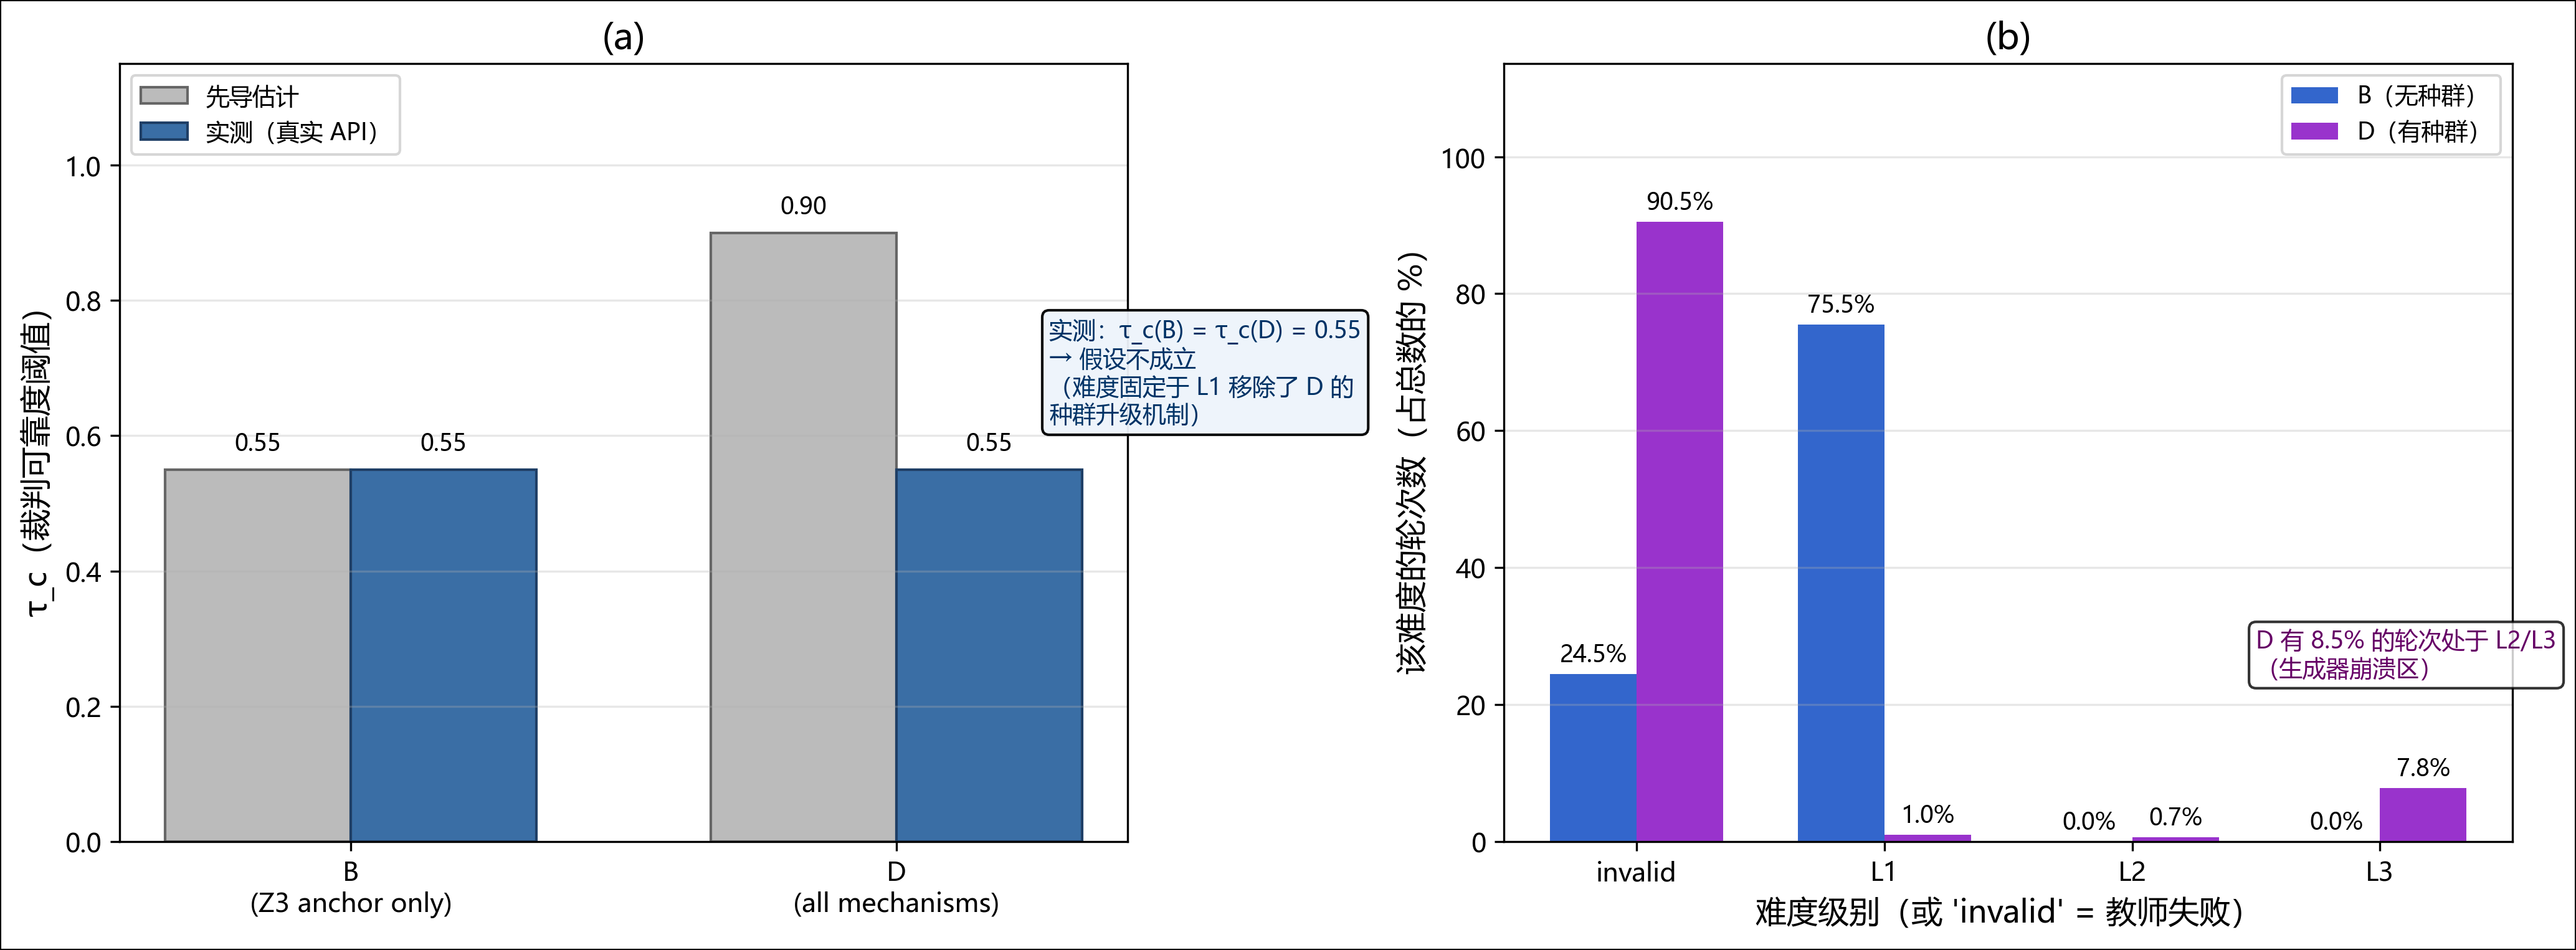
\includegraphics[width=\textwidth]{figures_zh/fig7_tau_c_gap.png}
  \caption{一次先导性估计曾给出 $\tau_c(D) = 0.90$、$\tau_c(B) = 0.55$；实测
  并未重现该差距（二者均为 0.55）。左图把先导估计与实测的 $\tau_c$ 并置
  对比，右图比较 B 与 D 的难度分布。假设
  $\tau_c(D) > \tau_c(B)$ \textit{未获支持}。}
  \label{fig:tau_c_gap}
\end{figure*}

\begin{figure*}[t]
  \centering
  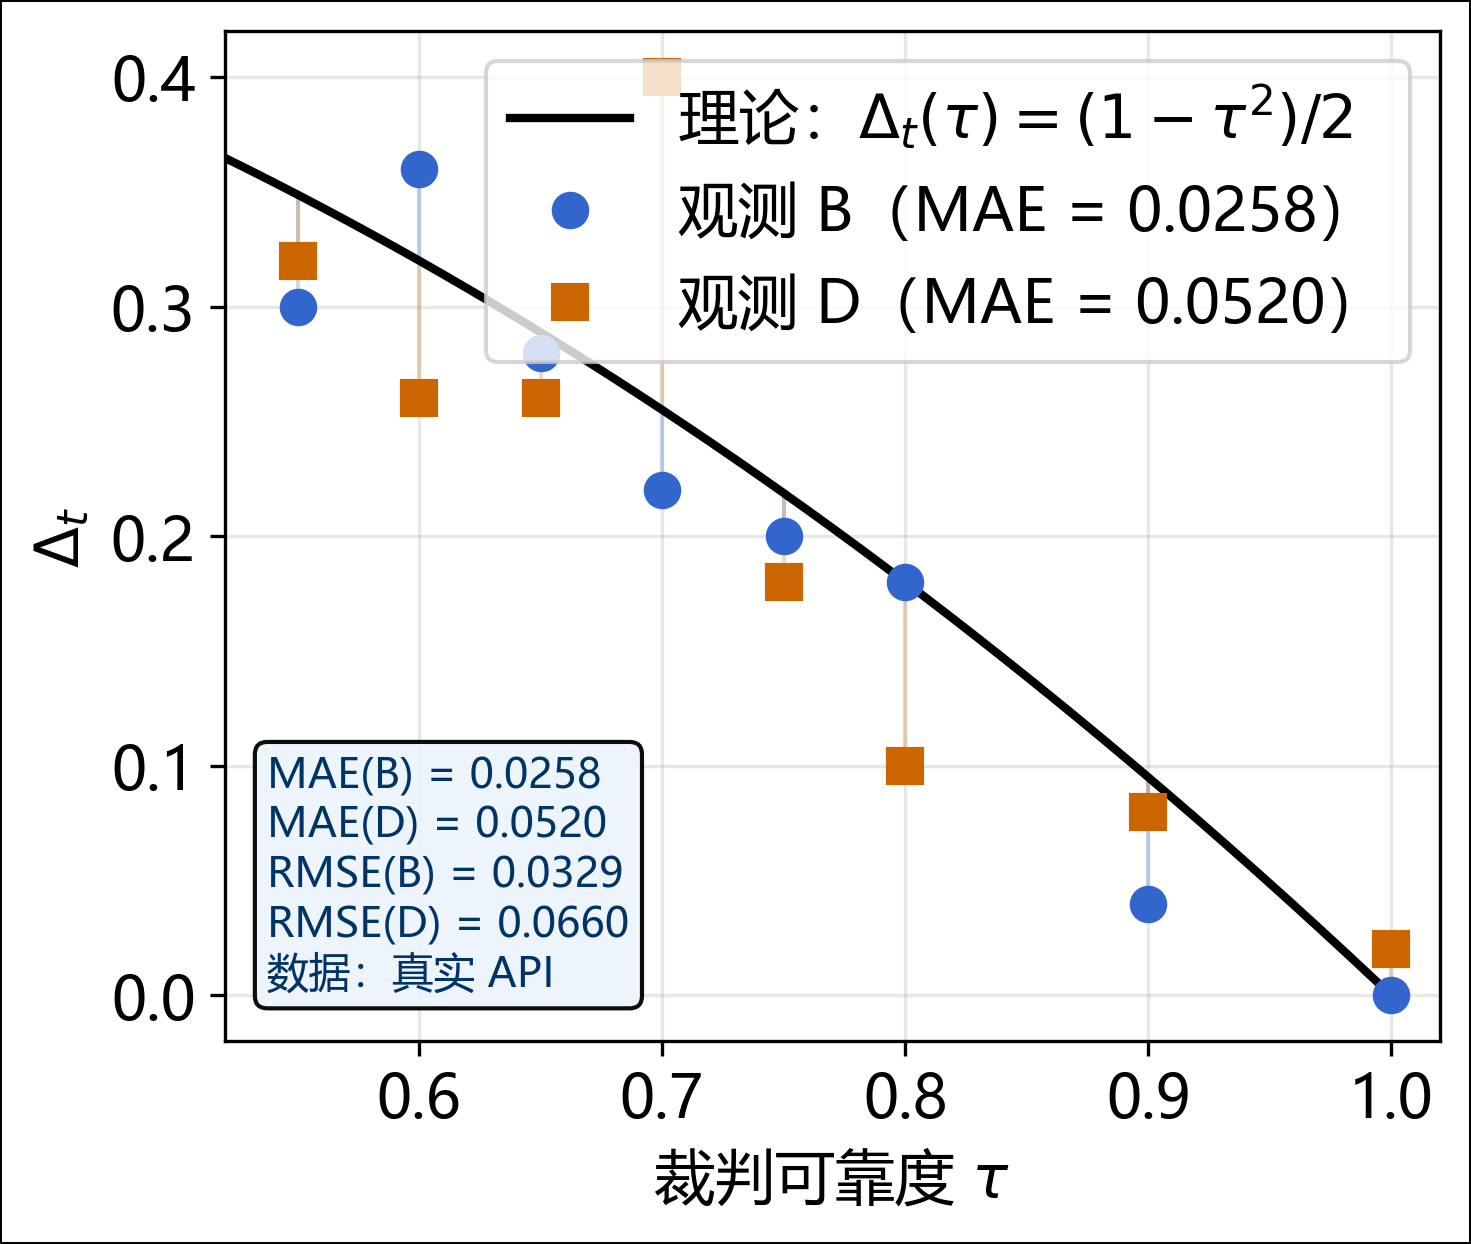
\includegraphics[width=\textwidth]{figures_zh/fig5b_tau_c_analytical.png}
  \caption{闭式解 $\Delta_t(\tau) = (1 - \tau^2)/2$ 与观测散点的对照。该
  公式不含自由参数；在每个 $\tau$ 格子上以 50 轮测得的 MAE 为 0.0258（B）
  与 0.0520（D）。当 $\tau = 0$ 时曲线锚定于 0.5 而非 1.0，这正是两次
  独立裁决所构成的二元对称性。}
  \label{fig:analytical_fit_appendix}
\end{figure*}

\begin{figure*}[t]
  \centering
  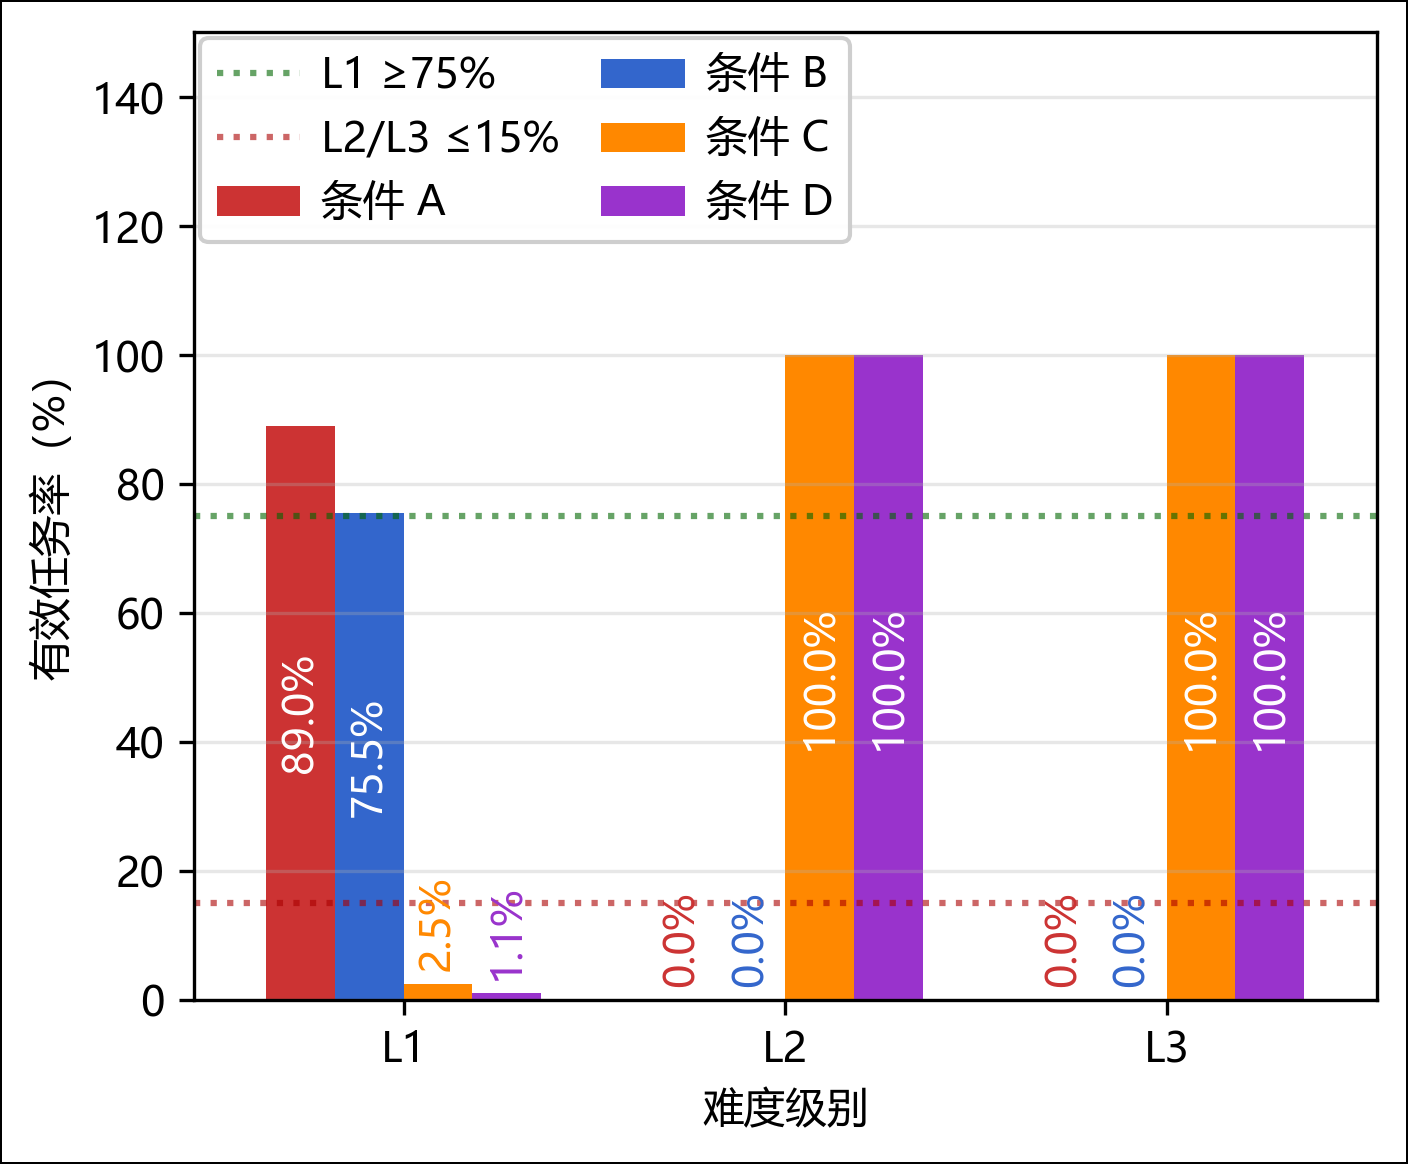
\includegraphics[width=\textwidth]{figures_zh/fig3b_validity_by_level.png}
  \caption{按难度层级划分的有效任务率。每一个抵达 L2/L3 的轮次都产出了
  有效任务：C 与 D 的 85.5\% 与 90.5\% 无效率发生在层级指派\textit{之前}，
  因为教师在 L1$\to$L2 过渡处失败，而控制器却把层级维持在高位。
  这就是伪难度陷阱。}
  \label{fig:validity_by_level_appendix}
\end{figure*}

\begin{figure*}[t]
  \centering
  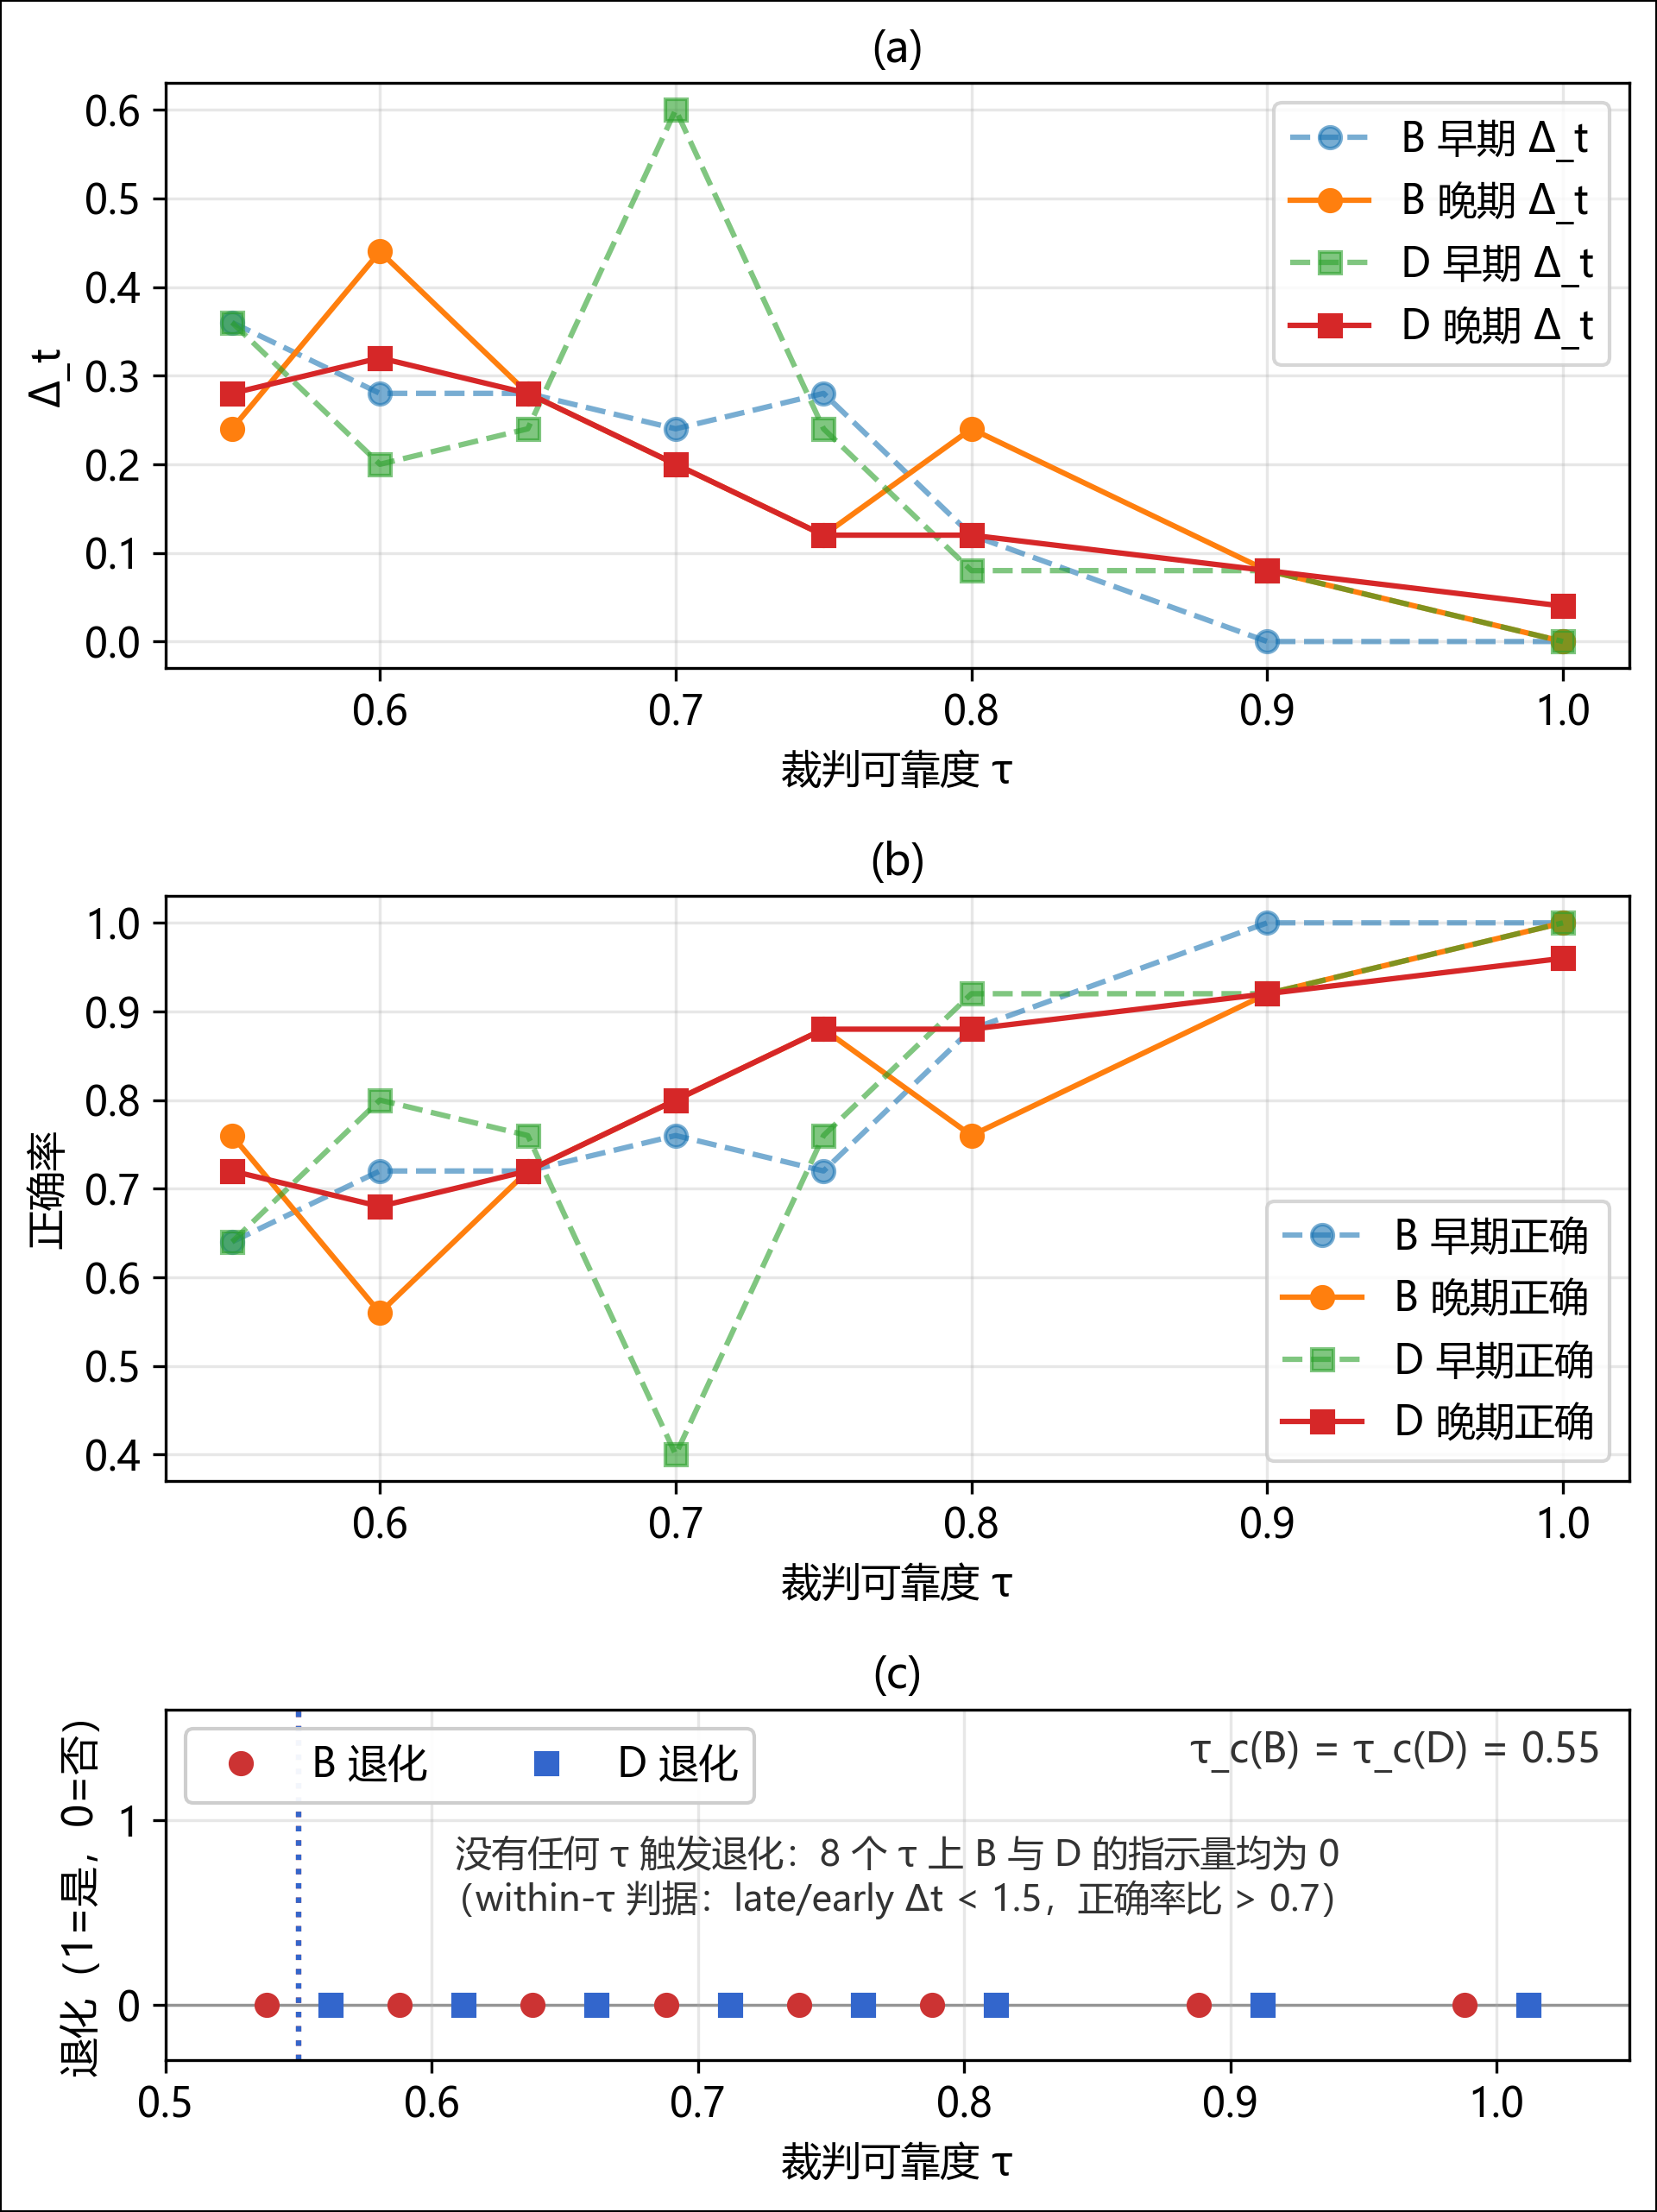
\includegraphics[width=\textwidth]{figures_zh/fig5_tau_c_curve_real.png}
  \caption{真实 API 上的 $\tau$ 梯度扫描：8 个 $\tau$ 取值 $\times$ 2 个条件（B/D）
  $\times$ 50 轮 = 800 轮。在 $\tau$ 内退化判据下没有任何 $\tau$ 取值
  发生退化，因此所报告的 $\tau_c = 0.55$ 是扫描网格的下边缘，应
  理解为上界，而非系统的容差。子图 (c) 画的是退化指示量：它在八个 $\tau$ 上
  对两个条件均为 0；两条竖线标记
  $\tau_c(B) = \tau_c(D) = 0.55$。}
  \label{fig:tau_c_curve_appendix}
\end{figure*}

\begin{figure*}[t]
  \centering
  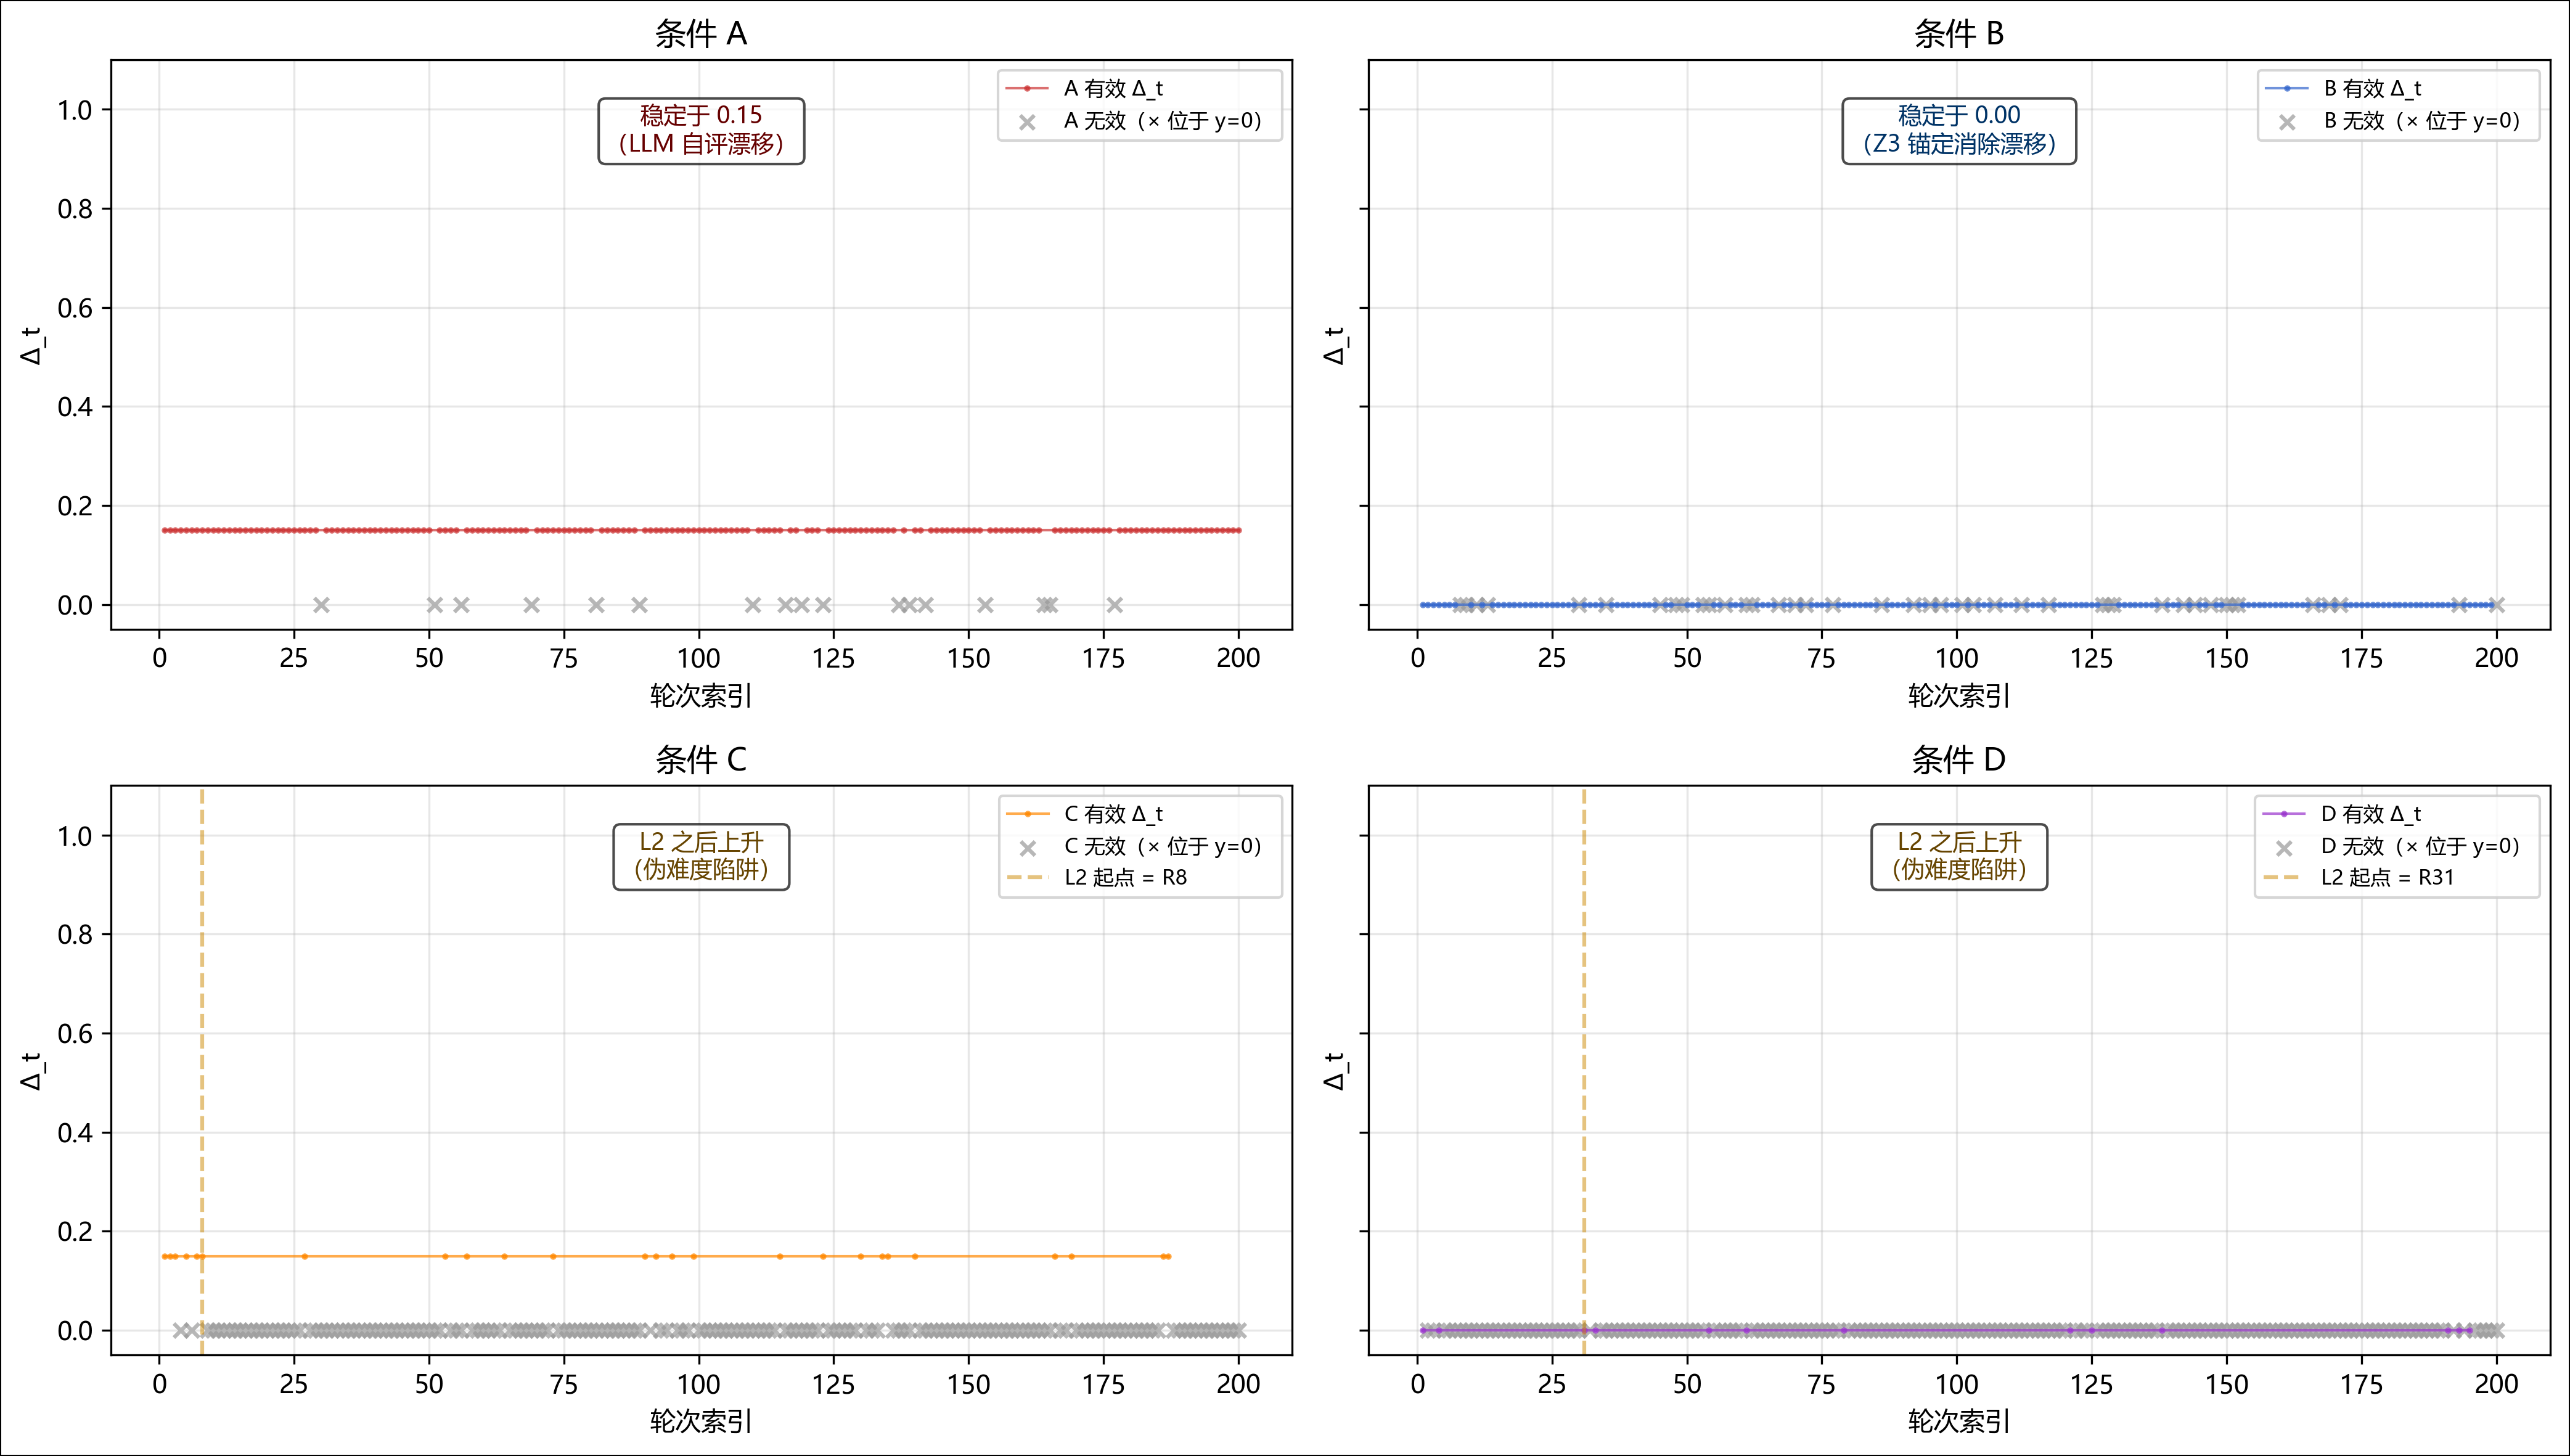
\includegraphics[width=\textwidth]{figures_zh/fig2b_delta_t_per_round.png}
  \caption{每个子图对应一个条件；无效轮次以灰色叉号标记。C/D 展示了
  L2 过渡之后的伪难度陷阱。竖线标记难度控制器首次
  提升任务层级的轮次。}
  \label{fig:delta_t_per_round_appendix}
\end{figure*}

\section{定理 1 证明梗概}

\subsection*{合成律的代数推导}

% 注：任务书要求在“附录 B”下给出本推导。在既定结构中附录 B
% 的标题是“定理 1 证明梗概”，因此这里以子节形式给出这段推导。
% 若该附录应独立成篇，可对其重命名。

令 $S = 1$ 表示该轮成功（有效任务且判定正确），否则为 $0$。令 $G = 1$
表示生成器产出有效任务，否则为 $0$；令 $J = 1$ 表示裁判正确评估
该轮次，否则为 $0$。于是 $S = G \cdot J$。由独立性（independence）：
\[
  \mathbb{E}[S] = \mathbb{E}[G] \cdot \mathbb{E}[J]
\]
\[
  1 - \Delta_t^{\mathrm{global}} = (1 - \Delta_t^{\mathrm{gen}})(1 - \Delta_t^{\mathrm{valid}})
\]

